\documentclass[14pt]{extbook}
\usepackage{multicol, enumerate, enumitem, hyperref, color, soul, setspace, parskip, fancyhdr} %General Packages
\usepackage{amssymb, amsthm, amsmath, bbm, latexsym, units, mathtools} %Math Packages
\everymath{\displaystyle} %All math in Display Style
% Packages with additional options
\usepackage[headsep=0.5cm,headheight=12pt, left=1 in,right= 1 in,top= 1 in,bottom= 1 in]{geometry}
\usepackage[usenames,dvipsnames]{xcolor}
\usepackage{dashrule}  % Package to use the command below to create lines between items
\newcommand{\litem}[1]{\item#1\hspace*{-1cm}\rule{\textwidth}{0.4pt}}
\pagestyle{fancy}
\lhead{Progress Quiz 3}
\chead{}
\rhead{Version B}
\lfoot{3148-2249}
\cfoot{}
\rfoot{Spring 2021}
\begin{document}

\begin{enumerate}
\litem{
Write the equation of the line in the graph below in Standard form $Ax+By=C$. Then, choose the intervals that contain $A, B, \text{ and } C$.
\begin{center}
    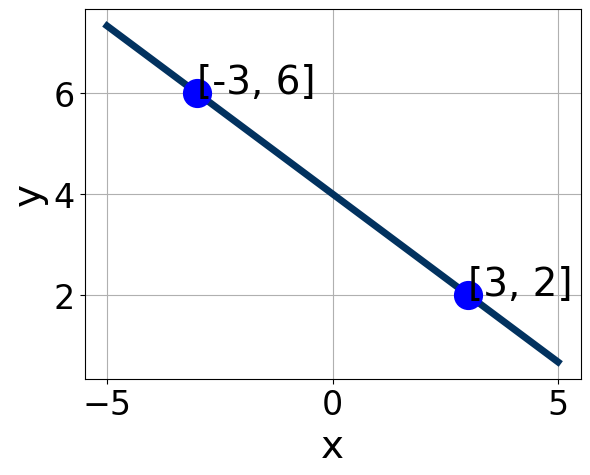
\includegraphics[width=0.5\textwidth]{../Figures/linearGraphToStandardCopyB.png}
\end{center}
\begin{enumerate}[label=\Alph*.]
\item \( A \in [-0.5, 1.8], \hspace{3mm} B \in [-0.65, 2.42], \text{ and } \hspace{3mm} C \in [-1.8, -0.4] \)
\item \( A \in [1, 4.9], \hspace{3mm} B \in [4.55, 5.7], \text{ and } \hspace{3mm} C \in [-6.5, -3.6] \)
\item \( A \in [1, 4.9], \hspace{3mm} B \in [-5.19, -3.45], \text{ and } \hspace{3mm} C \in [4.7, 7.2] \)
\item \( A \in [-0.5, 1.8], \hspace{3mm} B \in [-1.07, -0.63], \text{ and } \hspace{3mm} C \in [0.4, 4.2] \)
\item \( A \in [-3.2, -0.2], \hspace{3mm} B \in [-5.19, -3.45], \text{ and } \hspace{3mm} C \in [4.7, 7.2] \)

\end{enumerate} }
\litem{
Solve the equation below. Then, choose the interval that contains the solution.\[ -5(-18x -4) = -14(-9x -16) \]\begin{enumerate}[label=\Alph*.]
\item \( x \in [-5.13, 2.87] \)
\item \( x \in [4.78, 10.78] \)
\item \( x \in [-5.67, -4.67] \)
\item \( x \in [-6.78, -5.78] \)
\item \( \text{There are no real solutions.} \)

\end{enumerate} }
\litem{
Solve the equation below. Then, choose the interval that contains the solution.\[ -12(9x + 16) = -3(-6x + 13) \]\begin{enumerate}[label=\Alph*.]
\item \( x \in [-2.94, -2.3] \)
\item \( x \in [-2.55, -1.5] \)
\item \( x \in [-1.65, -1.07] \)
\item \( x \in [0.42, 2.59] \)
\item \( \text{There are no real solutions.} \)

\end{enumerate} }
\litem{
Find the equation of the line described below. Write the linear equation as $ y=mx+b $ and choose the intervals that contain $m$ and $b$.\[ \text{Perpendicular to } 7 x - 4 y = 12 \text{ and passing through the point } (-5, -3). \]\begin{enumerate}[label=\Alph*.]
\item \( m \in [-1.6, -0.2] \hspace*{3mm} b \in [-6.86, -3.86] \)
\item \( m \in [-1.6, -0.2] \hspace*{3mm} b \in [3.86, 9.86] \)
\item \( m \in [-1.6, -0.2] \hspace*{3mm} b \in [2, 4] \)
\item \( m \in [-0.1, 3.3] \hspace*{3mm} b \in [-1.14, 0.86] \)
\item \( m \in [-4.7, -1.7] \hspace*{3mm} b \in [-6.86, -3.86] \)

\end{enumerate} }
\litem{
Find the equation of the line described below. Write the linear equation as $ y=mx+b $ and choose the intervals that contain $m$ and $b$.\[ \text{Perpendicular to } 4 x + 7 y = 5 \text{ and passing through the point } (9, 6). \]\begin{enumerate}[label=\Alph*.]
\item \( m \in [0.68, 2.58] \hspace*{3mm} b \in [-5, -2] \)
\item \( m \in [0.68, 2.58] \hspace*{3mm} b \in [-11.75, -4.75] \)
\item \( m \in [0.68, 2.58] \hspace*{3mm} b \in [9.75, 11.75] \)
\item \( m \in [-2.18, -0.97] \hspace*{3mm} b \in [21.75, 27.75] \)
\item \( m \in [0.35, 1] \hspace*{3mm} b \in [-11.75, -4.75] \)

\end{enumerate} }
\litem{
First, find the equation of the line containing the two points below. Then, write the equation as $ y=mx+b $ and choose the intervals that contain $m$ and $b$.\[ (6, 5) \text{ and } (5, -5) \]\begin{enumerate}[label=\Alph*.]
\item \( m \in [8, 11] \hspace*{3mm} b \in [55, 56] \)
\item \( m \in [-10, -9] \hspace*{3mm} b \in [42, 49] \)
\item \( m \in [8, 11] \hspace*{3mm} b \in [-1, 7] \)
\item \( m \in [8, 11] \hspace*{3mm} b \in [-57, -51] \)
\item \( m \in [8, 11] \hspace*{3mm} b \in [-11, -8] \)

\end{enumerate} }
\litem{
Write the equation of the line in the graph below in Standard form $Ax+By=C$. Then, choose the intervals that contain $A, B, \text{ and } C$.
\begin{center}
    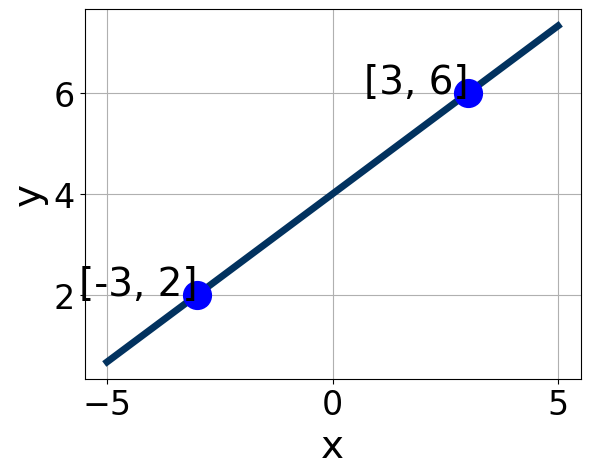
\includegraphics[width=0.5\textwidth]{../Figures/linearGraphToStandardB.png}
\end{center}
\begin{enumerate}[label=\Alph*.]
\item \( A \in [-1.3, 0.3], \hspace{3mm} B \in [-1.3, -0.76], \text{ and } \hspace{3mm} C \in [-6, -3] \)
\item \( A \in [0.8, 2.9], \hspace{3mm} B \in [-3.59, -2.38], \text{ and } \hspace{3mm} C \in [-14, -10] \)
\item \( A \in [-2.1, -1.9], \hspace{3mm} B \in [2.99, 3.06], \text{ and } \hspace{3mm} C \in [12, 15] \)
\item \( A \in [-1.3, 0.3], \hspace{3mm} B \in [0.32, 2.37], \text{ and } \hspace{3mm} C \in [1, 6] \)
\item \( A \in [0.8, 2.9], \hspace{3mm} B \in [2.99, 3.06], \text{ and } \hspace{3mm} C \in [12, 15] \)

\end{enumerate} }
\litem{
Solve the linear equation below. Then, choose the interval that contains the solution.\[ \frac{-3x -3}{7} - \frac{-3x -5}{4} = \frac{3x -7}{6} \]\begin{enumerate}[label=\Alph*.]
\item \( x \in [-3.87, -1.87] \)
\item \( x \in [50.4, 54.4] \)
\item \( x \in [0.66, 3.66] \)
\item \( x \in [9.13, 16.13] \)
\item \( \text{There are no real solutions.} \)

\end{enumerate} }
\litem{
Solve the linear equation below. Then, choose the interval that contains the solution.\[ \frac{-7x + 6}{3} - \frac{-8x -3}{7} = \frac{-5x + 7}{4} \]\begin{enumerate}[label=\Alph*.]
\item \( x \in [-37.6, -32.6] \)
\item \( x \in [-2.11, 0.89] \)
\item \( x \in [-15.4, -6.4] \)
\item \( x \in [3, 4] \)
\item \( \text{There are no real solutions.} \)

\end{enumerate} }
\litem{
First, find the equation of the line containing the two points below. Then, write the equation as $ y=mx+b $ and choose the intervals that contain $m$ and $b$.\[ (8, -4) \text{ and } (-2, 6) \]\begin{enumerate}[label=\Alph*.]
\item \( m \in [-1.5, -0.5] \hspace*{3mm} b \in [-4, -1] \)
\item \( m \in [-0.1, 3.3] \hspace*{3mm} b \in [7, 13] \)
\item \( m \in [-1.5, -0.5] \hspace*{3mm} b \in [3, 6] \)
\item \( m \in [-1.5, -0.5] \hspace*{3mm} b \in [-13, -5] \)
\item \( m \in [-1.5, -0.5] \hspace*{3mm} b \in [7, 13] \)

\end{enumerate} }
\end{enumerate}

\end{document}